%%%%%%%%%%%%%%%%%%%%%%%%%%%%%%%%%%%%%%%%%%%%%%%%%%%%%%%%%%%%%%%%%%%%%%%%%%%%%%%%
% University of Western Ontario Thesis Template
% By: Justin Quinn Veenstra, 2010
% With thanks to Mr. (soon to be Dr.) Will Robertson.


\documentclass[12pt,twoside]{report}

%%%%%%%%%%%%%%%%%%%%%%%%%%%%%%%%%%%%%%%%%%%%%%%%%%%%%%%%%%%%%%%%%%%%%%%%
%%                                                                    %%
%%                    ***   I M P O R T A N T   ***                   %%
%%                                                                    %%
%% Fill in the following fields with the required information:        %%
%%  - \department{Department of Psychology.}  name of the graduate department               %%
%%  - \degree{Masters of Science}      name of the degree obtained                   %%
%%  - \author{Avital Sternin}      name of the author                            %%
%%  - \title{...}       title of the thesis                           %%
%%  - \gyear{2016}       year of graduation                            %%
%%  - \super{Dr. Jessica A. Grahn & Dr. Adrian M. Owen}    supervisor
%%  - \firstname, \middlename, \lastname... there is additional documentation by the actual fields, so I'll leave it at that
%%%%%%%%%%%%%%%%%%%%%%%%%%%%%%%%%%%%%%%%%%%%%%%%%%%%%%%%%%%%%%%%%%%%%%%%
\usepackage{appendix}
\usepackage{graphicx}
\usepackage{amsmath}
%\numberwithin{figure}{chapter}
\usepackage[byname]{smartref}
\usepackage{booktabs,tabularx} % nicer tables
\usepackage{soul}
\usepackage{hyperref} %comment out for hardcopy
\hypersetup{linkcolor=blue, citecolor=blue, colorlinks=true}  % Colours hyperlinks in blue, but this can be distracting if there are many links.
\usepackage{apacite} %THIS HAS TO GO AFTER HYPERREF 

\usepackage{acronym}
\acrodef{EEG}{electroencephalography}
\acrodef{ICA}{independent component analysis}
\acrodef{ERP}{event-related potential}
\acrodef{PCA}{principle component analysis}
\acrodef{CAE}{convolutional auto-encoder}
\acrodef{CNN}{convolutional neural network}
\acrodef{MSRE}{mean squared reconstruction error}
\acrodef{MIR}{music information retrieval}
\acrodef{BCI}{brain-computer interface}
\acrodef{SSEP}{steady state evoked potential}

\newcommand{\etal}{et al.~}


\usepackage{txfonts}
\usepackage{tocloft}
\makeatletter

\def\@makechapterhead#1{%
  %%%%\vspace*{50\p@}% %%% removed!
  {\parindent \z@ \raggedright \normalfont
    \ifnum \c@secnumdepth >\m@ne
        \huge\bfseries \@chapapp\space \thechapter
        \par\nobreak
        \vskip 20\p@
    \fi
    \interlinepenalty\@M
    \Huge \bfseries #1\par\nobreak
    \vskip 40\p@
  }}
\def\@makeschapterhead#1{%
  %%%%%\vspace*{50\p@}% %%% removed!
  {\parindent \z@ \raggedright
    \normalfont
    \interlinepenalty\@M
    \Huge \bfseries  #1\par\nobreak
    \vskip 40\p@
  }}

\newenvironment{acknowledgements}%
{\clearemptydoublepage
 \begin{center}
  \section*{Acknowledgements}
 \end{center}
 \begingroup
}{\newpage\endgroup}

\newenvironment{dedication}%
{\clearemptydoublepage 
 \begin{center}
  \section*{Dedication}
 \end{center}
 \begingroup
}{\newpage\endgroup}

\newenvironment{preliminary}%
{\pagestyle{plain}\pagenumbering{roman}}%
{\pagenumbering{arabic}}

% Default values for title page.

%% To produce output with the desired line spacing, the argument of
%% \spacing should be multiplied by 5/6 = 0.8333, so that 1 1/2 spaced
%% corresponds to \spacing{1.5} and double spaced is \spacing{1.66}.
\def\normalspacing{1.25} % default line spacing


%% Define the "thesis" page style.
\if@twoside % If two-sided printing.
\def\ps@thesis{\let\@mkboth\markboth
   \def\@oddfoot{}
   \let\@evenfoot\@oddfoot
   \def\@oddhead{
      {\sc\rightmark} \hfil \rm\thepage
      }
   \def\@evenhead{
      \rm\thepage \hfil {\sc\leftmark}
      }
   \def\chaptermark##1{\markboth{\ifnum \c@secnumdepth >\m@ne
      Chapter\ \thechapter. \ \fi ##1}{}}
   \def\sectionmark##1{\markright{\ifnum \c@secnumdepth >\z@
      \thesection. \ \fi ##1}}}
\else % If one-sided printing.
\def\ps@thesis{\let\@mkboth\markboth
   \def\@oddfoot{}
   \def\@oddhead{
      {\sc\rightmark} \hfil \rm\thepage
      }
   \def\chaptermark##1{\markright{\ifnum \c@secnumdepth >\m@ne
      Chapter\ \thechapter. \ \fi ##1}}}
\fi

\pagestyle{thesis}
% Set up page layout.
\setlength{\textheight}{9in} % Height of the main body of the text
\setlength{\topmargin}{-.5in} % .5" margin on top of page
\setlength{\headsep}{.5in}  % space between header and top of body
\addtolength{\headsep}{-\headheight} % See The LaTeX Companion, p 85
\setlength{\footskip}{.5in}  % space between footer and bottom of body
\setlength{\textwidth}{6.25in} % width of the body of the text
\setlength{\oddsidemargin}{.25in} % 1.25" margin on the left for odd pages
\setlength{\evensidemargin}{0in} % 1.25"  margin on the right for even pages

% Marginal notes
\setlength{\marginparwidth}{.75in} % width of marginal notes
\setlength{\marginparsep}{.125in} % space between marginal notes and text

% Make each page fill up the entire page. comment this out if you
% prefer. 
%\flushbottom

\setcounter{tocdepth}{3} % Number the subsubsections 
\def\normalspacing{1.25} % default line spacing

\newcommand\isco[1]{%
  \edef\@tempa{#1}%
  \def\@tempb{}%
  \ifx\@tempa\@tempb
	\else \\\underline{Co-Supervisor:}\vspace{0.35in}\\\dots\dots\dots\dots\dots\dots\dots\\{#1}\\
  \fi
}

\newcommand\isjoint[1]{%
  \edef\@tempa{#1}%
  \def\@tempb{}%
  \ifx\@tempa\@tempb
	\else \\\underline{Joint Supervisor:}\vspace{0.35in}\\\dots\dots\dots\dots\dots\dots\dots\\{#1}\\
  \fi
}

\newcommand\isalt[1]{%
  \edef\@tempa{#1}%
  \def\@tempb{}%
  \ifx\@tempa\@tempb
	\else \\\underline{Alternate Supervisor:}\vspace{0.35in}\\\dots\dots\dots\dots\dots\dots\dots\\{#1}\\
  \fi
}

\newcommand\isdefinedsig[1]{%
  \edef\@tempa{#1}%
  \def\@tempb{}%
  \ifx\@tempa\@tempb
	\else \\ \dots\dots\dots\dots\dots\dots\dots\\{#1}\\
  \fi
}
\newcommand\isdefinedspinetitle[1]{%
  \edef\@tempa{#1}%
  \def\@tempb{}%
  \ifx\@tempa\@tempb
	\else (Spine title: #1)\\
  \fi
}
\newcommand\coauthor[1]{%
  \edef\@tempa{#1}%
  \def\@tempb{}%
  \ifx\@tempa\@tempb
	\else \newpage \Large Co-Authorship Statement\normalsize\\\indent\\#1\\
  \fi
}

\newcommand\acknowlege[1]{%
  \edef\@tempa{#1}%
  \def\@tempb{}%
  \ifx\@tempa\@tempb
	\else \newpage \Large Acknowlegements\normalsize\\\indent\\#1\newpage
  \fi
}

%\renewcommand{\appendixtocname}{\Huge \textbf{List of Appendices} \normalsize}
\newcommand{\blank}{\hspace{-2mm}}
\newcommand{\super}{Dr. Jessica A. Grahn} %supervisor
\newcommand{\superj}{Dr. Adrian M. Owen} %joint supervisor, if there is one, leave blank if not (lbin)... only one of the three.
\newcommand{\superc}{} %co-supervisor, if there is one, leave blank if not (lbin)
\newcommand{\supera}{} %alternate supervisor, if there is one, leave blank if not (lbin)
\newcommand{\sco}{}  %member of supervisory committee
\newcommand{\sct}{}  %other member of supervisory committee (lbin)
\newcommand{\examo}{Dr. Marc Joanisse}  %examining committee (up to four, if less leave blank)
\newcommand{\examt}{Dr. Ingrid Johnsrude}
\newcommand{\examth}{Dr. Mark Daley}
\newcommand{\examf}{}
\newcommand{\department}{Department of Psychology}
\newcommand{\degree}{Masters of Science}
\newcommand{\firstname}{Avital}
\newcommand{\middlename}{}
\newcommand{\lastname}{Sternin}
%\renewcommand{\author}[1]{\ifx\empty#1\else\gdef\@author{#1}\fi} 
\newcommand{\authorname}{{\firstname} {\middlename} {\lastname}}
\newcommand{\titl}{Classifying music perception and imagination from EEG}
\newcommand{\spinetitle}{Plib}%only if the above is more than 60 characters
\newcommand{\thesisformat}{Monograph} %or Integrated Article
\newcommand{\gyear}{\number\year}
%\newcommand{\makecoauthor}{
%Type information about coauthorship here/ }
\newcommand{\makeacknowlege} {
%Type in acknowlegements here
}
\newcommand{\listappendixname}{List of Appendices}
\newlistof{myappendices}{app}{\listappendixname}
\newcommand{\myappendices}[1]{%
\addcontentsline{app}{myappendices}{#1}\par}

\renewcommand{\maketitle}
{\begin{titlepage}
   \setcounter{page}{1}
   %% Set the line spacing to 1 for the title page.
   %\begin{spacing}{1} 
   \begin{large}
   \begin{center}
      \mbox{}
      \vfill
      {\MakeUppercase{\titl}}\\
      \isdefinedspinetitle{\spinetitle}
      (Thesis format: \thesisformat)\\
      \vfill
      by \\
      \vfill
      {\firstname} \underline{\lastname}\\
      \vfill
      Graduate Program in {\department}\\
      \vfill
		A thesis submitted in partial fulfillment\\
		of the requirements for the degree of\\
		\degree\\
		\vfill
		The School of Graduate and Postdoctoral Studies\\
		The University of Western Ontario\\
		London, Ontario, Canada\\
		\vfill
      {\copyright} {\authorname} {\gyear}  \\
      \vspace*{.2in}
   \end{center}
   \end{large}
%   \end{spacing}
   \end{titlepage}

}%\maketitle

\newcommand{\makecert}{
   \setcounter{page}{2}
\vfill
\begin{center}
\large
THE UNIVERSITY OF WESTERN ONTARIO\\
School of Graduate and Postdoctoral Studies\\
\vfill
\textbf{CERTIFICATE OF EXAMINATION}
\end{center}

\vfill
\begin{table}[ht]
\begin{minipage}[t]{0.5\linewidth} %tabular instead?
\begin{tabular}{l}
\underline{Supervisor:}\vspace{0.35in}
\isdefinedsig{\super}
\isco{\superc}
\isjoint{\superj}
\isalt{\supera}
\\
\underline{Supervisory Committee:}\vspace{0.35in}
\isdefinedsig{\sco}\vspace{0.15in}
\isdefinedsig{\sct}
\end{tabular}
\vfill
\end{minipage}
\hspace{0.5in}
\begin{minipage}[t]{0.5\linewidth}
\begin{tabular}{l}
\underline{Examiners:} \\\vspace{.5cm}
\isdefinedsig{\examo}\\
\isdefinedsig{\examt}\\
\isdefinedsig{\examth}\\
\isdefinedsig{\examf}
\end{tabular}
\vfill
\end{minipage}
\vfill
\end{table}
\vfill
\begin{center}
The thesis by \\ \vfill
\textbf{\firstname{} \middlename{} \underline{\lastname}}\\
\vfill
entitled:\\\vfill
\textbf{\titl}\\\vfill
is accepted in partial fulfillment of the \\
requirements for the degree of\\
\degree\\
\end{center}
\begin{table}[ht]
\begin{minipage}[t]{0.5\linewidth}
\begin{tabular}{l}
\dots\dots\dots\dots\dots\\
Date
\end{tabular}
\end{minipage}
\hspace{0.5in}
\begin{minipage}[t]{0.5\linewidth}
\begin{tabular}{l}
\dots\dots\dots\dots\dots\dots\dots\dots\dots\dots\\
Chair of the Thesis Examination Board
\end{tabular}
\end{minipage}
\end{table}

}

\makeatother
\begin{document}

%% ***   NOTE   ***
%% You should put all of your '\newcommand', '\newenvironment', and
%% '\newtheorem's (in other words, all the global definitions that you
%% will need throughout your thesis) in a separate file and use
%% "\input{filename}" to input it here.


%% This sets the page style and numbering for preliminary sections.
\begin{preliminary}

%% This generates the title page from the information given above.
\maketitle
\addcontentsline{toc}{chapter}{Certificate of Examination}
\makecert
\newpage
%\addcontentsline{toc}{chapter}{Co-Authorship Statement}
%\coauthor{\makecoauthor}  %comment this out if none
%\newpage
%\addcontentsline{toc}{chapter}{Acknowlegements}
%\acknowlege{\makeacknowlege}	%as above
\addcontentsline{toc}{chapter}{Abstract}
\Large\begin{center}\textbf{Abstract}\end{center}\normalsize
%%  ***  Put your Abstract here.   ***
%% (150 words for M.Sc. and 350 words for Ph.D.)

This is a really silly abstract.

\vfill
\textbf{Keywords:} Time series analysis, data mining
\newpage
\tableofcontents
\newpage
\addcontentsline{toc}{chapter}{List of Figures}
\listoffigures
\newpage
\addcontentsline{toc}{chapter}{List of Tables}
\listoftables\newpage
\addcontentsline{toc}{chapter}{List of Appendices}
\listofmyappendices\newpage
%\addcontentsline{toc}{chapter}{List of Abbreviations, Symbols, and Nomenclature}
%\large List of Abbreviations, Symbols, and Nomenclature \normalsize
%\newpage
\end{preliminary}
%% End of the preliminary sections: reset page style and numbering.

\chapter*{Introduction}
\addcontentsline{toc}{chapter}{1. Introduction}

Everybody imagines music. Imagining music can be defined as a deliberate internal recreation of the perceptual experience of listening to music \cite{schaefer_name_2011}.
Individuals can imagine themselves producing music, imagine listening to others produce music, or simply "hear" the music in their heads. 
Music imagination is used by musicians to memorize music and anyone who has ever had an "ear-worm" -- a tune stuck in their head -- has experienced imagining music. Because of its simplicity no training is required to imagine a song, and researchers have been investing the utility of music imagery for \acp{BCI}.
A \ac{BCI} is a system that allows an external device to be controlled or modified using brain activity. 
Music imagery appears to be a very promising means for driving \acp{BCI} that use \ac{EEG} -- a popular non-invasive neuroimaging technique that relies on electrodes placed on the scalp to measure the electrical activity of the brain.
For instance, Schaefer \etal\cite{schaefer_measuring_2011} argue that
\emph{``music is especially suitable to use here as (externally or internally generated) stimulus material, since it unfolds over time, and \ac{EEG} is especially precise in measuring the timing of a response.''}
For patients that have difficulties communicating behaviourally (e.g. patients with locked-in syndrome) \ac{BCI}s are a promising communication tool. 
{BCI}s that currently exist are generally binary systems that allow the user to choose between two options to answer yes/no questions. %limiting communication abilities. 
A system with a larger number of answer options would offer a more complete communication experience. 
Using music as the basis for a \ac{BCI} is a promising way to build such a system due to the large number of musical pieces that exist. 
Ideally, a music-based \ac{BCI} would allow the user to imagine a piece of music in order to convey a particular thought. 
However, the translation from music imagination will require careful processing of the EEG data. 

EEG data contain a variety of signals, elicited by sounds, that can be exploited by a \ac{BCI}. 
%However, the EEG data is full of unwanted signals (noise) and extracting the relevant information can be a challenge.
%Decoding brain wave recordings to classify different states is a relatively new field of research.
%A recent review of neuroimaging methods for \ac{MIR} that also covers techniques different from EEG is given in \cite{ismir2015kaneshiro}.
\ac{EEG} signals have been used to measure emotions induced by music perception \cite{lin_eeg_2009,cabredo_emotion_2012} and to distinguish perceived rhythmic stimuli \cite{stober2014nips}.
Further in the rhythmic domain it has been shown that oscillatory neural activity in the gamma frequency band (20-60 Hz) is sensitive to accented tones in a rhythmic sequence \cite{snyder_gamma-band_2005}.
Oscillations in the beta band (20-30 Hz) entrain to rhythmic sequences \cite{cirelli_beta_2014, merchant_beta_2015} and increase in anticipation of strong tones in a non-isochronous, rhythmic sequence \cite{iversen_top-down_2009,fujioka_beta_2009,fujioka_internalized_2012}.
The magnitude of \acp{SSEP}, which reflect neural oscillations entrained to the stimulus, changes when subjects hear rhythmic sequences for frequencies related to the metrical structure of the rhythm.
This is a sign of entrainment to beat and meter \cite{nozaradan_tagging_2011,nozaradan_selective_2012}. 
\ac{EEG} studies have further shown that perturbations of the rhythmic pattern lead to distinguishable \acp{ERP} \cite{geiser_early_2009}.
Furthermore, Vlek \etal \cite{vlek_shared_2011} showed that imagined auditory accents imposed on top of a steady metronome click can be recognized from EEG.

Recently studies have identified a close relationship between the brain areas that are active during the imagination and the perception of music \cite{halpern_fmri_2004,Kraemer2005,Herholz2008,herholz_2012}. 
Although not directly relevant to a \ac{BCI}, we can learn a lot from \ac{EEG} data collected while participants listen to melodies.
Exploring EEG data during music perception can inform how we approach music imagination data and the brain signals recorded while listening to music could serve as reference data to determine which salient elements are to be expected during imagination. 
By using perception data as a way to train our \ac{BCI} we can cut down on the amount of imagination training needed which will reduce potential user fatigue.

EEG has already successfully been used to classify perceived melodies. 
In a study by Schaefer \etal \cite{schaefer_name_2011}, 10 participants \textit{listened} to 7 short melody clips with a length between 3.26s and 4.36s.
For single-trial classification, each stimulus was presented 140 times in randomized back-to-back sequences of all stimuli.
Using a quadratically regularized linear logistic-regression classifier with 10-fold cross-validation, they were able to successfully classify the \acp{ERP} of single trials.
Within subjects, the accuracy varied between 25\% and 70\%.
Applying the same classification scheme across participants, they obtained between 35\% and 53\% accuracy.
%In a further analysis, they combined all trials from all subjects and stimuli into a grand average \ac{ERP}.
%Using singular-value decomposition, they obtained a fronto-central component that explained 23\% of the total signal variance.
%The time courses corresponding to this component showed significant differences between stimuli that were strong enough to allow cross-participant classification.
%As Hubbard concludes in his recent review of the literature on auditory imagery, \emph{``auditory imagery preserves many structural and temporal properties of auditory stimuli''} and \emph{``involves many of the same brain areas as auditory perception''} \cite{hubbard_auditory_2010}. 
%This is also underlined by Schaefer \cite[p. 142]{schaefer_measuring_2011} whose \emph{``most important conclusion is that there is a substantial amount of overlap between the two tasks} [music perception and imagination]\emph{, and that `internally' creating a perceptual experience uses functionalities of `normal' perception.''}

Brain activity during music imagination has also been detected by \ac{EEG} \cite{schaefer_shared_2013}, and encouraging preliminary results for recognizing imagined music fragments from \ac{EEG} recordings were reported in \cite{schaefer_single_2009} in which 4 out of 8 participants produced imagery that was classifiable (in a binary comparison) with an accuracy between 70\% and 90\% after 11 trials.

Although \ac{EEG} has been used to decode music imagination the accuracy levels are not robust enough for these decoding techniques to be used in a \ac{BCI}. 
This could be because the EEG processing methods may not be sensitive enough to the subtle changes that occur during music imagination. 
The sophisticated signal processing techniques used in machine learning can lend expertise to this challenge. 

Machine learning is a technique that uses algorithms that can learn from and make predictions about data.
For example, the programs used by postal services to recognize handwriting on envelopes or the speech recognition software in your cell phone are based on machine learning techniques.
One such technique is based on convolutional neural networks (\acp{CNN}).
\acp{CNN} were inspired by the powerfully complex visual system found in humans and other animals.
In the retina we have cells that are responsive to small regions of the visual field \cite{hubel_receptive_1963}. 
As information moves along the visual processing stream and into the brain single cells in higher layers receive input from multiple cells in lower layers.
At each level of this process more information is combined.
This gives cells higher up in the processing stream an increasingly global view of what information was collected by the retinal cells.
Complex visual information is processed farther along the processing stream than simple information as cells in these far layers are sent information from a larger number of retinal cells.
\acp{CNN} work in a similar way to process complex data. 
The processing units in a \ac{CNN} act like cells in the visual system.
The ``receptive field'' of each one of these units is determined by a filter.
Each filter is created based on a variety of parameters set by the researcher or determined by the network during the training process.
%In this experiment the filters used are \acp{CAE} (as described in \cite{masci_stacked_2011}).
%A \ac{CAE} is an artificial neural network that is able to extract features from data without supervision.
% feature extractor that scales well to high dimensional input.
%CAEs are a special variant of a \ac{CNN} that encode their input using convolution into a compressed internal representation. 
%This representation is then decoded using de-convolution into the original space while trying to minimize the reconstruction error. 
%This type of neural network can learn a meaningful but compressed representation of the data.
%Importantly, \acp{CAE} preserve spatial information allowing them to learn biologically plausible features.%
%Once the \ac{CAE} has extracted the important features from the training data and constructed the filters these filters can be used in a \ac{CNN}.
%These filters are very similar to the components produced in \ac{PCA} and \ac{ICA} with the difference being the parameters used to compute the components. 
%The \ac{CAE} filters aim to minimize the \ac{MSRE} rather than the orthogonality or independence criteria used in \ac{PCA} and \ac{ICA} respectively. 
Before a \ac{CNN} can be used to classify data it must learn the characteristics of the data. 
The \ac{CNN} is trained using a subset of the data and the filters are optimized to produce the best classification results. 
The optimized filters are applied to new data and the accuracy of the classification is determined. 

%SUMMARY OF WHAT WE TRIED AND THE TECHNIQUES WE USED
%Using this analysis technique we aim to be able to classify what a participant was listening to or imagining based on the signal in their EEG data alone. 
To approach this problem we first tried an ERP analysis similar to that of Schaefer \etal\cite{schaefer_name_2011} in order to determine which piece of music a participant was listening to or imagining.
When this proved unsuccessful we used a machine learning technique called deep learning to detect more subtle differences in the EEG that would be more useful in classifying stimuli. 
Using this technique we were able to classify perception of 12 music pieces with a 28.7\% accuracy (chance=8.3\%).
We were unable to accurately classify imagination of music \hl{specific values go here}.
\section*{Methods}
\addcontentsline{toc}{chapter}{Methods}
\subsection*{Participants}
Fourteen participants (3 male), aged 19-36, with normal hearing and no history of brain injury took part in this study. Eight participants had formal musical training (1- 26 years), and four of the participants played instruments regularly at the time of data collection.
\vspace{-0.5em}
\subsection*{Stimuli}
Stimuli were fragments of familiar musical pieces and were selected based on key signature (3/4 or 4/4 time) and the presence and absence of lyrics. The stimuli were kept as similar in length as possible with care taken to ensure that they all contained complete musical phrases. Stimulus details can be found in \autoref{tab:stimuli_information}.
Each musical fragment was preceded by approximately two seconds of clicks as a cue to the tempo and onset of the music. The beats began to fade out at the one second mark and stopped at the onset of the music. 
\begin{table}[t]
%\vspace{-1em}
\setlength{\tabcolsep}{2.5pt}  % use to control space between columns
\renewcommand{\arraystretch}{1}
\centering
\caption{Information about the tempo, meter and length of the stimuli used in this experiment.}
%Mean and standard deviation over individual subjects.}
\label{tab:stimuli_information}
{\footnotesize % \sffamily \fontfamily{anttlc}\selectfont
%{\small % \sffamily \fontfamily{anttlc}\selectfont
\begin{tabularx}{\columnwidth}{r l c c  c c c }
\toprule
ID		& Name							&Meter 	& Length	& Tempo 		&\#Bars	& Bar Length\\
\midrule
1		& Chim Chim Cheree (lyrics)			& 3/4		& 13.3s 			& 212 BPM 	& 16				& 0.85s	\\ % ($\ge$12 bars)\\
2		& Take Me Out to the Ballgame (lyrics)	& 3/4		& 7.7s 			& 189 BPM 	& 8				& 0.95s	\\ % ($\ge$9 bars)\\
3		& Jingle Bells (lyrics)					& 4/4		& 9.7s 			& 200 BPM 	& 8				& 1.20s	\\ % ($\ge$12 bars)\\
4		& Mary Had a Little Lamb (lyrics)		& 4/4		& 11.6s			& 160 BPM 	& 8				& 1.50s	\\ % ($\ge$12 bars)\\
11		& Chim Chim Cheree 				& 3/4		& 13.5s	 		& 212 BPM 	& 16				& 0.85s	\\ % ($\ge$12 bars)\\
12		& Take Me Out to the Ballgame			& 3/4		& 7.7s 			& 189 BPM 	& 8				& 0.95s	\\ % ($\ge$9 bars)\\
13		& Jingle Bells 						& 4/4		& 9.0s 			& 200 BPM 	& 8				& 1.20s	\\ % ($\ge$12 bars)\\
14		& Mary Had a Little Lamb				& 4/4		& 12.2s			& 160 BPM 	& 8				& 1.50s	\\ % ($\ge$12 bars)\\
21		& Emperor Waltz					& 3/4		& 8.3s 			& 178 BPM 	& 8				& 1.01s	\\ % ($\ge$12 bars)\\
22		& Hedwig's Theme (Harry Potter)		& 3/4		& 16.0s	 		& 166 BPM 	& 15				& 1.08s	\\ % ($\ge$9 bars)\\
23		& Imperial March (Star Wars Theme)		& 4/4		& 9.2s 			& 104 BPM 	& 4				& 2.30s	\\ % ($\ge$12 bars)\\
24		& Eine Kleine Nachtmusik				& 4/4		& 6.9s			& 140 BPM 	& 4				& 1.71s	\\ % ($\ge$12 bars)\\
\bottomrule
\end{tabularx}
}
%\vspace{-1em}
%\vspace{-0.8em}
\end{table}

\subsection*{Equipment and Procedure}
\subsubsection*{Behavioural Testing}
We collected information about the participants' previous music experience, their ability to imagine sounds, and information about musical sophistication using an adapted version of the widely used Goldsmith's Musical Sophistication Index (G-MSI) \cite{mullensiefen_musicality_2014} combined with an adapted clarity of auditory imagination scale \cite{willander_imagery_scale_2010}. 
We also had participants complete a beat tapping and a stimuli familiarity task. 
Participants listened to each stimulus and were asked to tap along with the music on the table top. The experimenter then rated their tapping ability on a scale from 1 (difficult to assess) to 3 (tapping done properly). 
After listening to each stimulus participants rated their familiarity with the stimuli on a scale from 1 (unfamiliar) to 3 (very familiar).
To participate in the \ac{EEG} portion of the study, the participants had to receive a score of at least 90\% on our beat tapping task. Participants received scores from 75\%--100\% with an average score of 96\%.
Furthermore, they needed to receive a score of at least 80\% on our stimuli familiarity task. 
Participants received scores from 71\%--100\% with an average score 87\%.
These requirements resulted in rejecting 4 participants.
This left 10 participants (3 male), aged 19--36, with normal hearing and no history of brain injury. 
These 10 participants had an average tapping score of 98\% and an average familiarity score of 92\%.
Eight participants had formal musical training (1--10 years), and four of those participants played instruments regularly at the time of data collection.

\subsubsection*{EEG recording}
For the EEG portion of the study, the 10 participants were seated in an audiometric room (Eckel model CL-13) and connected to a BioSemi Active-Two system recording 64+2 EEG channels at 512 Hz as shown in \autoref{fig:eegsetup}.
\begin{figure}
  \begin{center}
    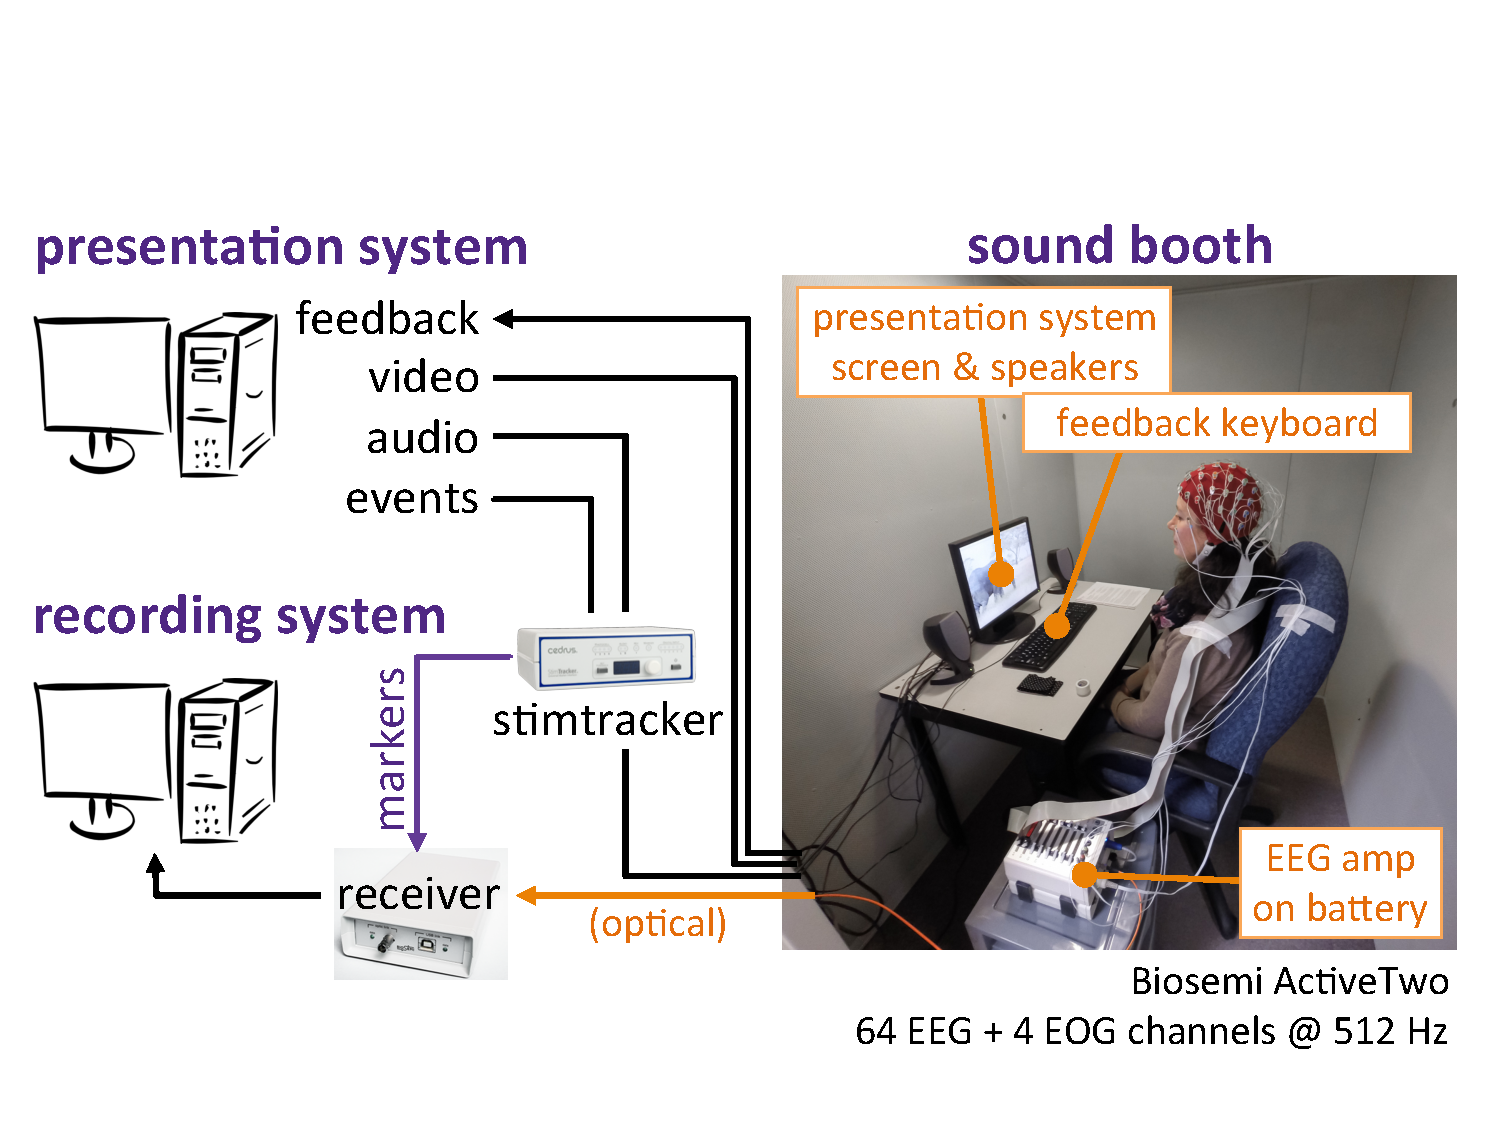
\includegraphics[width=\columnwidth,keepaspectratio=true]{Figures/EEG-setup.pdf}
%   \\\vspace{-0.8em}
    \caption{%
Setup for the EEG experiment.
The presentation and recording systems were placed outside to reduce the impact of electrical line noise that could be picked up by the EEG amplifier.
}
    \label{fig:eegsetup}
  \end{center}
% \vspace{-2em}
\end{figure}
Horizontal and vertical EOG channels were used to record eye movements. 
We also recorded the left and right mastoid channel as EEG reference signals. 
Due to an oversight, the mastoid data was not collected for the first 5 subjects.
The presented audio %and the recorded EEG were 
was routed through a Cedrus StimTracker connected to the EEG receiver, which allowed a high-precision synchronization ($<$0.05 ms) of the stimulus onsets with the \ac{EEG} data.
The experiment was programmed and presented using PsychToolbox run in Matlab 2014a. 
A computer monitor displayed the instructions and fixation cross for the participants to focus on during the trials to reduce eye movements.
The stimuli and cue clicks were played through speakers at a comfortable volume that was kept constant across participants. Headphones were not used because pilot participants reported headphones caused them to hear their heartbeat which interfered with the imagination portion of the experiment. 
After the experiment, we asked participants the method they used to imagine music. 
The participants were split evenly between imagining themselves producing the music (singing or humming) and simply ``hearing the music in [their] head.'' 

The EEG experiment was divided into 2 parts with 5 blocks each as illustrated in \autoref{fig:experiment_outline}.
% Note: 	the figure won't be place exactly here (this would require [h]. [t] stands for "top")
%			This just makes sure, it comes after the 1st reference
\begin{figure*}
  \begin{center}
    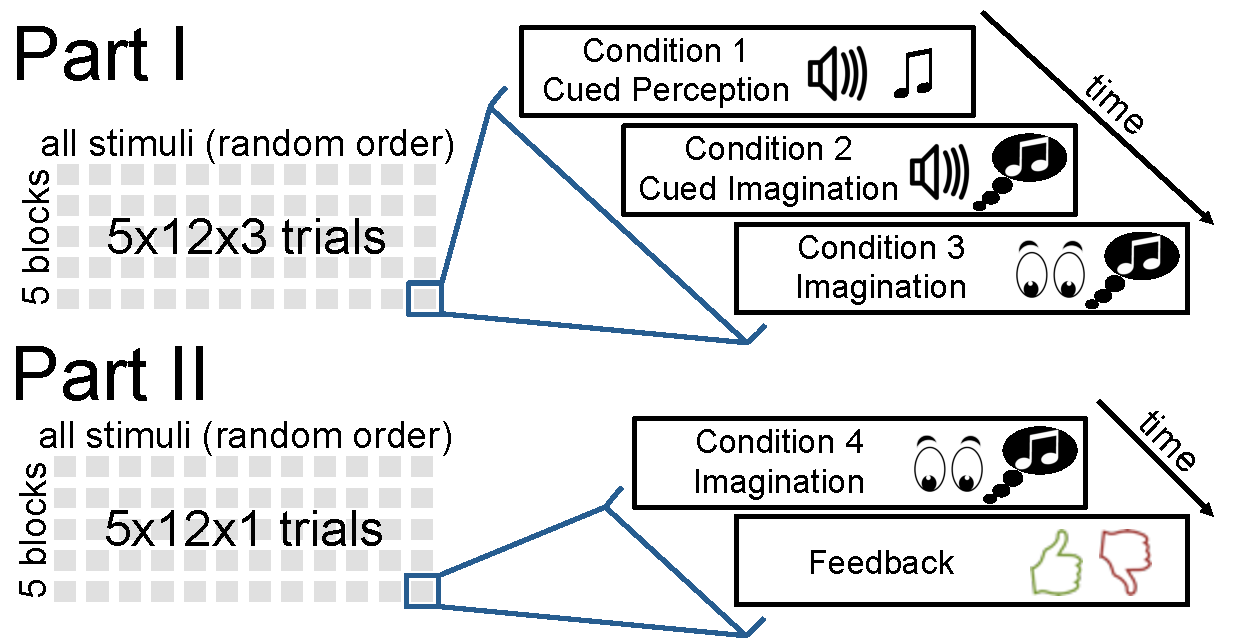
\includegraphics[width=0.8\textwidth,keepaspectratio=true]{Figures/study_design_small.pdf}
%   \\\vspace{-0.8em}
    \caption{%
Illustration of the design for the EEG portion of the study.
}
    \label{fig:experiment_outline}
  \end{center}
%  \vspace{-2em}
\end{figure*}

A single block comprised of all 12 stimuli in randomized order.
Between blocks, participants could take breaks at their own pace.
We recorded EEG in 4 conditions:
\begin{enumerate}
\item
Stimulus perception preceded by cue clicks
\item
Stimulus imagination preceded by cue clicks
\item
Stimulus imagination without cue clicks
\item
Stimulus imagination without cue clicks, with feedback
\end{enumerate}
The goal was to use the cue to align trials of the same stimulus collected under conditions 1 and 2. Lining up the trials allows us to directly compare the perception and imagination of music and to identify overlapping features in the data. 
Conditions 3 and 4 simulate a more realistic query scenario during which the system does not have prior information about the tempo and meter of the imagined stimulus.
These two conditions were identical except for the trial context.
While the condition 1--3 trials were recorded directly back-to-back within the first part of the experiment, 
all condition 4 trials were recorded separately in the second part, without any cue clicks or tempo priming by prior presentation of the stimulus.
After each condition 4 trial, participants provided feedback by pressing one of two buttons indicating on whether or not they felt they had imagined the stimulus correctly.
In total, 240 trials (12 stimuli x 4 conditions x 5 blocks) were recorded per subject.
%
The event markers recorded in the raw EEG comprise:
\begin{itemize}
\item
	Trial labels (as a concatenation of stimulus ID and condition) at the beginning of each trial
\item
	Exact audio onsets for the first cue click of each trial in conditions 1 and 2 (detected by the Stimtracker)
\item
	Subject feedback for the condition 4 trials (separate event IDs for positive and negative feedback)
\end{itemize}	


%We are interested in estimating the tempo of the music stimuli from the EEG signal. 
%Our analyses here focus on the data gathered during the three conditions in the first block of the experiment. Participants reported that they were not confident in their performance on the trials collected from the second block of the experiment, therefore the data were excluded from analyses and will require further attention. %
%Basic EEG preprocessing techniques were used to remove artifacts and a dynamic beat tracker was used to estimate average tempo. 
%Autocorrelation curves were computed to investigate the periodicity seen in the average EEG waveforms and the peaks from these curves were found to be proportional to stimulus bar length. 
%To deal with the tempo variance that inevitably occurred during the music imagination trials, we used a sliding window to aggregate over all channels and computed a more accurate tempo value.

\subsection*{Preprocessing}
The raw EEG and EOG data were processed using the MNE-Python toolbox. 
For recordings with additional mastoid channels, the EEG data was re-referenced by subtracting the mean mastoid signal \cite{teplan_fundamentals_2002}.
We then removed and interpolated bad EEG channels identified by manual visual inspection.
For interpolation, the spherical splines method described in \cite{perrin_spherical_1989} was applied.
The data were then filtered with an fft-bandpass, keeping a frequency range between 0.5 and 30 Hz.
This also removed any slow signal drift in the EEG.
Afterwards, we down-sampled to a sampling rate of 64 Hz.
To remove artifacts caused by eye blinks, we computed independent components using extended Infomax \ac{ICA} \cite{lee_independent_1999} and semi-automatically removed components that had a high correlation with the EOG channels.
Finally, the 64 EEG channels were reconstructed from the remaining independent components without reducing dimensionality.
\include{Chapters/Tempo}
\chapter*{ERP Analysis}
\addcontentsline{toc}{chapter}{3. ERP Analysis}
%As proposed in \cite{schaefer_name_2011}, we computed grand average \acp{ERP} by aggregating over all trials (excluding the cue clicks) of the same stimulus from all subjects except P05 (due to the movement artifacts).
Our first analysis of the data followed a strategy similar to the one used in \cite{schaefer_name_2011}.
Schaefer \etal \cite{schaefer_name_2011} used very short stimuli (3.26s) allowing each stimulus to be repeated many times during during the experiment. 
This allowed them to average across hundreds of short trials. 
They then concatenated the grand average ERPs and applied a \ac{PCA}, which resulted in clearly defined spatial features. 
The differences in the time courses of these spatial features allowed for classification of their stimuli. 
We tried to replicate these results, but we had fewer repetitions of our stimuli. 
Therefore, to preserve as much data as possible we used the full length of the trials as opposed to the first 3.26 seconds. 
We computed grand average \acp{ERP}s by aggregating over the full length of all trials (excluding the cue) of the same stimulus from all subjects. 
We then concatenated the grand average \acp{ERP} and applied a \ac{PCA}. 
This resulted in principle components with poorly defined spatial components \autoref{fig:components} (A and B).

In order to preserve even more of the data and we took an alternative approach. 
All of the raw trials were concatenated to create a single, long trial that contained all of the raw EEG information.
We ran a \ac{PCA} on the concatenated raw trials without first calculating an average across trials. 
This produced clearly defined spatial components \autoref{fig:components} (C and D). 
Except for their (arbitrary) polarity the components are very similar across the two conditions, which replicates the results found in \cite{schaefer_name_2011}.

\begin{figure}[t] 
  \begin{center}
%    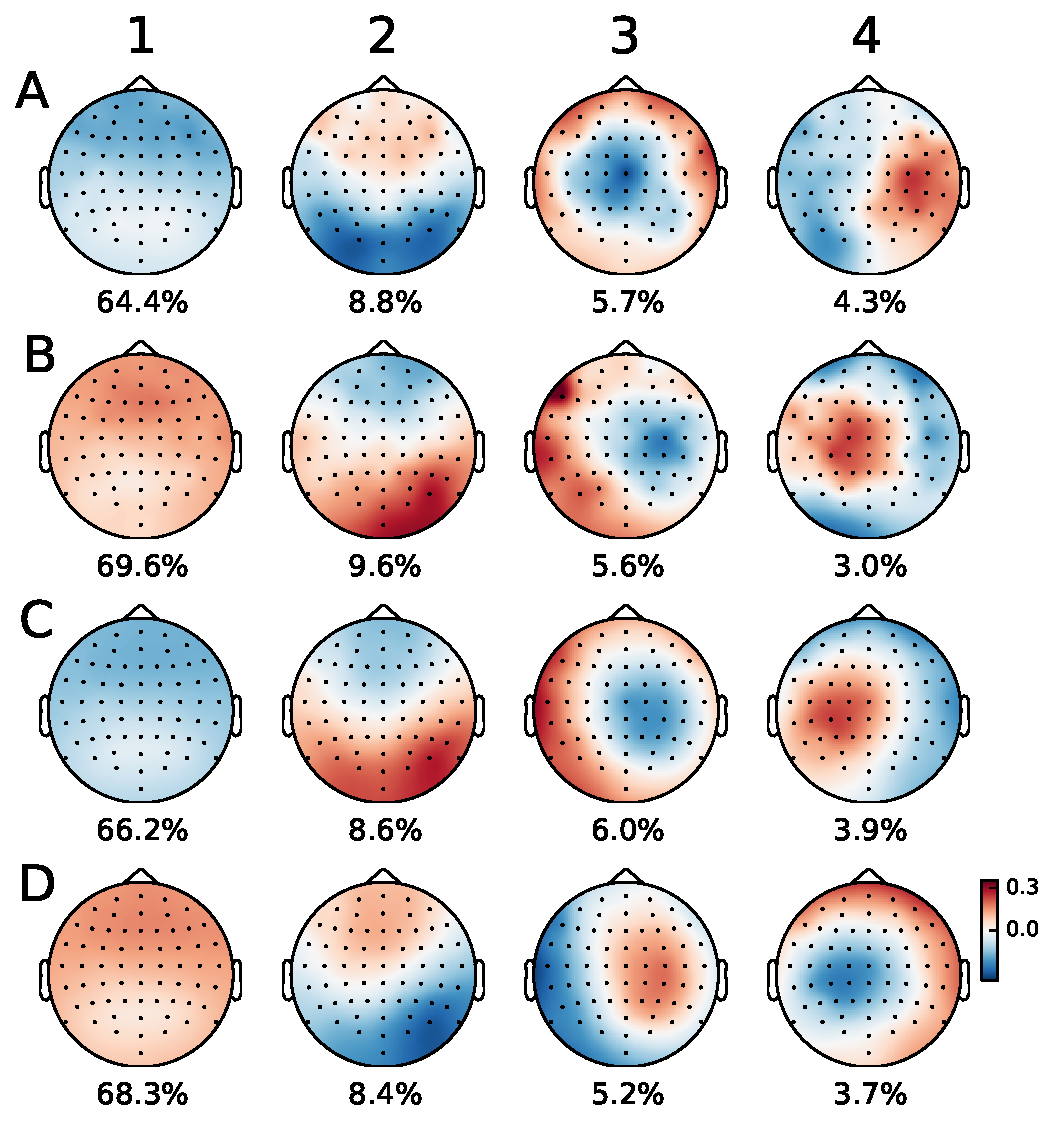
\includegraphics[width=0.8\textwidth,keepaspectratio=true]{Figures/principle_components.pdf}
    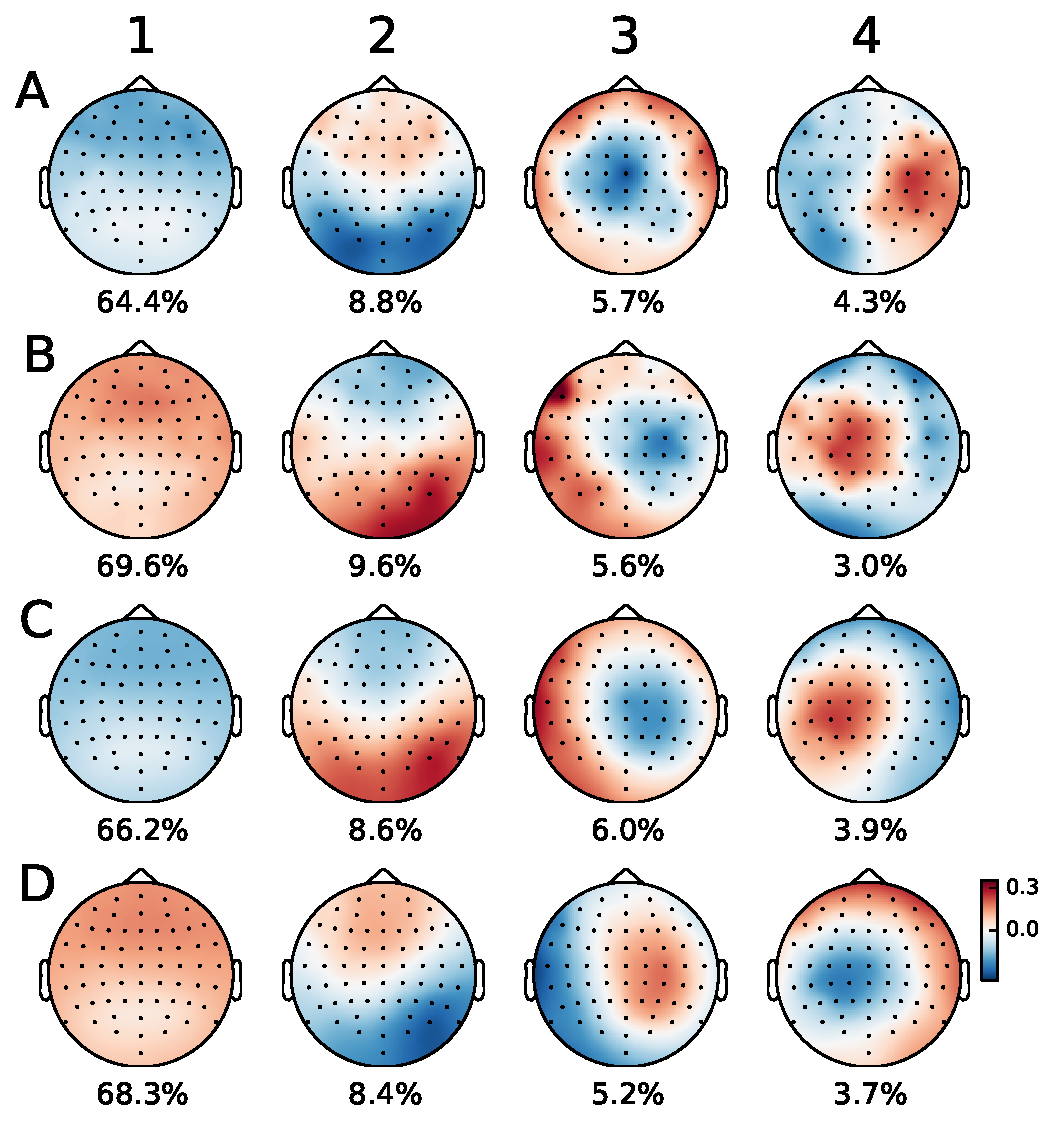
\includegraphics[scale=0.5]{Figures/principle_components.pdf}
%   \\\vspace{-0.8em}
    \caption{%
Topographic visualization of the top 4 principle components with percentage of the explained signal variance. %.\newline
Channel positions in the 64-channel EEG layout are shown as dots.
Colors are interpolated based on the channel weights.
%\hl{Polarity has no specific semantic.}
The PCA was computed on
\textbf{A}: the grand average \acp{ERP} of all perception trials,
\textbf{B}: the grand average \acp{ERP} of all cued imagination trials,
\textbf{C}: the concatenated perception trials,
\textbf{D}: the concatenated cued imagination trials.
}
    \label{fig:components}
  \end{center}
% \vspace{-2em}
\end{figure}

\subsection*{Component Waveform Correlations}
In order to investigate how similar the activation of these components is across conditions and stimuli we took the time course of component three over the first three seconds of each stimulus during perception and imagination and performed a correlation.
We used component three as it accounts for the most variance while being similar to a typical auditory component.
The highest correlations produced by this component is r=0.40 (p$<$0.001) for ``Eine Klein Nachtmusic'' (\autoref{fig:nachtmusic}) and r=0.30 (p$<$0.001) for ``The Emperor Waltz'' (\autoref{fig:emperor}).
Although these correlate well the perception of Eine Kleine Nachtmusic correlates well with the imagination of Jingle Bells without lyrics (r=0.30). 
The highest correlation of r=0.52 (p$<$0.001) occurs between the imagination of Jingle Bells (without lyrics) and the perception of the Star Wars theme \autoref{fig:starjingle}. 
Because high correlations occur between trials from different stimuli we can not use this approach to classify our stimuli.
\hl{include a Table of correlations? with Component 2? component 3?}

\begin{figure}[t]
  \begin{center}
    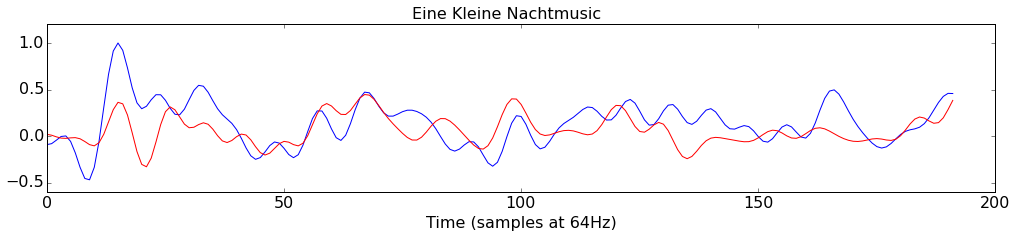
\includegraphics[scale=0.4]{Figures/EineKleineCorrelation}
    \caption{
The time course of component three during perception (blue) and imagination (red) of Eine Kleine Nachtmusic. The correlation between the two time courses is r=0.40 (p$<$0.001).
}
    \label{fig:nachtmusic}
  \end{center}
\end{figure}

\begin{figure}[t]
  \begin{center}
    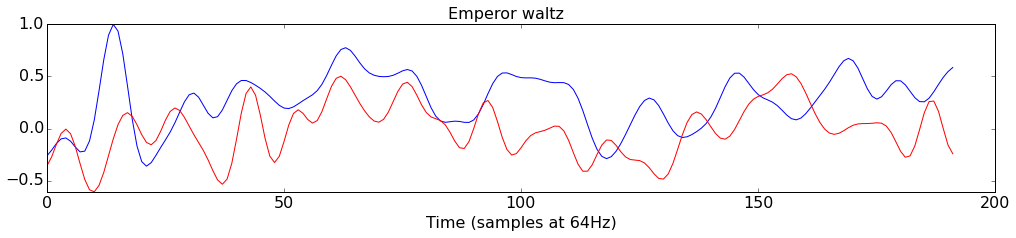
\includegraphics[scale=0.4]{Figures/EmperorCorrelation}
    \caption{
The time course of component three during perception (blue) and imagination (red) of The Emperor Waltz. The correlation between the two time courses is r=0.30 (p$<$0.001).
}
    \label{fig:emperor}
  \end{center}
\end{figure}

\begin{figure}[t]
  \begin{center}
    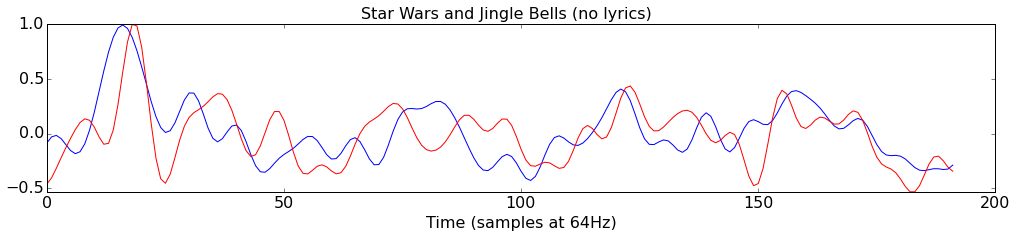
\includegraphics[scale=0.4]{Figures/StarJingle}
    \caption{
The time course of component three during perception (blue) of the Star Wars theme and imagination (red) of Jingle Bells (no lyrics). The correlation between the two time courses is r=0.52 (p$<$0.001).
}
    \label{fig:starjingle}
  \end{center}
\end{figure}

Our inability to accurately classify stimuli using this technique could be caused by our much smaller number of trials which are substantially longer than those used by \cite{schaefer_name_2011}. 
We only had 5 trials per stimulus, ranging from 6.9s to 16s, while Schaefer et al. (2011) collected 145 trials of each of their stimuli each approximately 3s long.
\chapter*{Classification}
\addcontentsline{toc}{chapter}{Classification}
Schaefer \etal \cite{schaefer_name_2011} were able to use the unique time course of the component responsible for the most variance to differentiate between stimuli.
Analyzing our components we have not yet been able to reproduce this significant stimulus classification accuracy. 
This could be caused by our much smaller number of trials which are substantially longer than those used by \cite{schaefer_name_2011}. 
On average we used \hl{X number of} trials in our analysis, while Schaefer et al. (2011) collected 145 trials of each of their stimuli.

We then attempted a different approach to classification using machine learning techniques. This approach facilitates better pattern learning by adapting components linked across subjects but that are also specific to each individual subject. 
We trained a \ac{CAE} as described in \cite{masci_stacked_2011} and implemented using pylearn2 \cite{goodfellow_pylearn2_2013}.
%CAEs are a special variant of a \ac{CNN} that encode their input using convolution into a compressed internal representation which is then decoded using de-convolution into the original space trying to minimize the reconstruction error. 
%Such a neural network can be used to learn a meaningful but compressed representation of the data. 
In this case the 64 \ac{EEG} channels were reduced to four combined channels -- each computed by a separate convolution filter. 
%These filters are very similar to the components produced in \ac{PCA} and \ac{ICA}. 
%The difference is the objective that is used to compute these components. 
%The \ac{CAE} filters aim to minimize the \ac{MSRE} using stochastic gradient descent over mini-batches rather than the orthogonality or independence criteria used in \ac{PCA} and \ac{ICA} respectively. 
\subsection*{Perception Classification Results}
First the \ac{CAE} was trained on all trials in the perception condition. The learned filter weights were then used as initialization values to create individual \ac{CAE}s specific to each participant.
The filters can be seen in \autoref{fig:components}. 
Minor differences between subjects can be seen. 

\begin{figure}[t]
  \begin{center}
    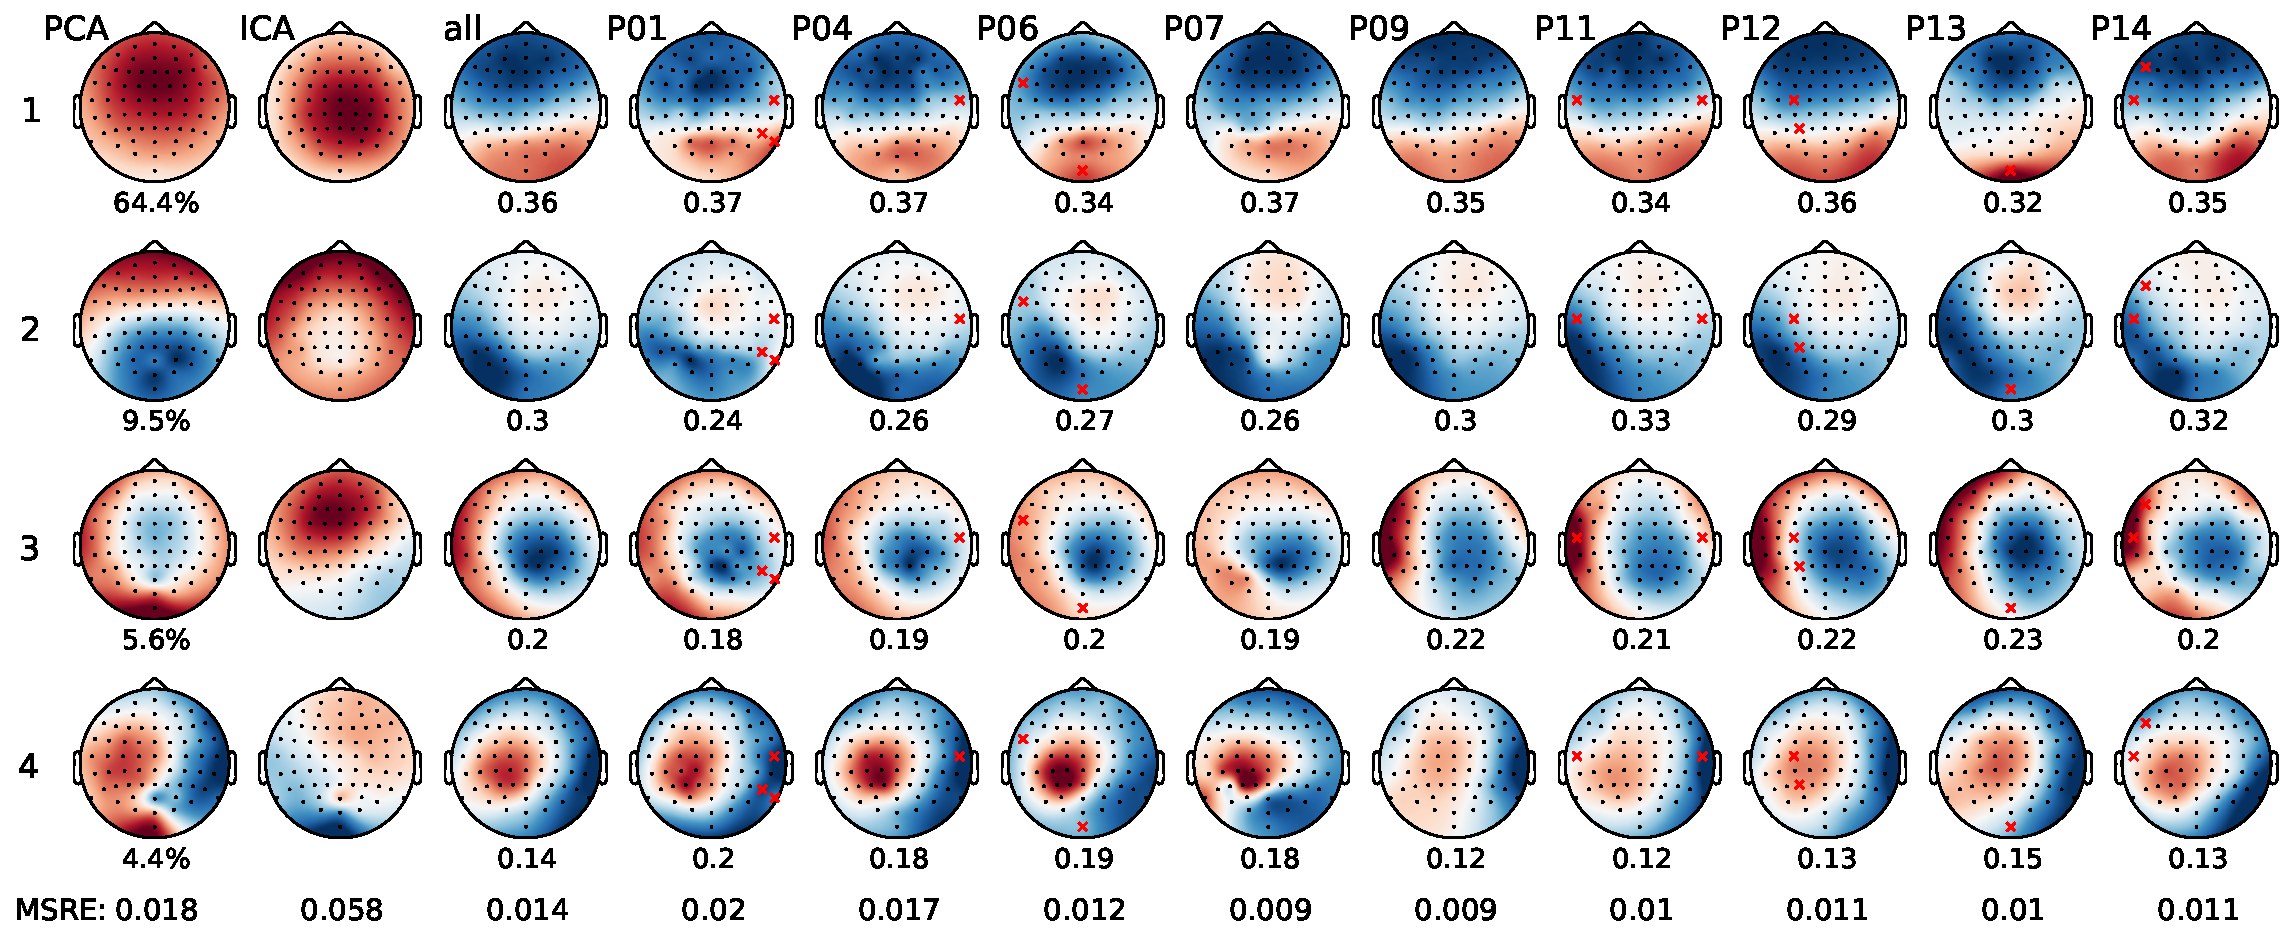
\includegraphics[width=\columnwidth,keepaspectratio=true]{Figures/topoplots_all.pdf}
    \caption{
Topographic map visualization of the EEG channel weights for the top 4 signal components derived from the perception trials. The leftmost two columns show the top 4 principal components (explaining over 87\% of the variance in total) and the corresponding independent components computed using extended Infomax ICA. The remaining columns show the weights learned by the convolutional auto-encoder for all subjects combined (third column) and all individual subjects labeled P01 to P14 accordingly. Numbers below the plots refer to the percentage of explained variance for principal components and the normalized biases for the filters of the convolutional auto-encoder respectively. Noisy EEG channels that were removed and interpolated are marked by red X?s. For subjects P09 to P14, mastoid channel referencing was applied. Values at the bottom of each column refer to the mean squared reconstruction error (MRSE) per sample.
}
    \label{fig:components}
  \end{center}
\end{figure}

We used the data from the learned components to train simple \ac{CNN}s with a single convolution layer and a \hl{DLSVM output layer} \cite{tang_deep_2013} on two classification tasks: stimulus identification (12 classes) and time-signature recognition (2 classes). 
We trained the CNN on 60\% of the trials. This same training set was used to train the \ac{CAE} prior to the \ac{CNN} training. 
The best model was selected using a validation set (20\% of trials) and it was evaluated on a test set (20\% of trials). 
\hl{We used dropout regularization} \cite{hinton_improving_2012}, momentum, and a linear learning rate decay over epochs.
A simple \ac{CNN} that used 16 [1x4]-convolution filters (over 1 sample in all 4 component activation channels) obtained 65.8\% (p=0.05) accuracy on the binary time-signature classification task. 
A CNN using 1 [16x4]-convolution filter (over 250ms in all 4 component activation channels with pooling for 140ms-windows and 5x sub-sampling obtained 19.5\% (p=0.001) on the 12 class stimulus recognition task. 
Significance values were determined by using the cumulative binomial distribution to estimate the likelihood of observing a given classification rate by chance.

\subsection*{Imagination Classification Results}
Imagination results from CNN. 

Table to summarize all results? 



%% This adds a line for the Bibliography in the Table of Contents.
\addcontentsline{toc}{chapter}{Bibliography}
%% ***   Set the bibliography style.   ***
\bibliographystyle{apacite} % (change according to your preference)
%%% ***   Set the bibliography file.   ***
\bibliography{Bibliography}{}
%% ***   NOTE   ***
%% If you don't use bibliography files, comment out the previous line
%% and use \begin{thebibliography}...\end{thebibliography}.  (In that
%% case, you should probably put the bibliography in a separate file
%% and \include or \input it here).

%Appendices.
\begin{appendices}
\chapter{Ethics Approval Form}\label{appendix:ethics}
\myappendices{Appendix \ref{appendix:ethics} {Ethics Approval Form}}

The Ethics Approval Form can be found on the following page.
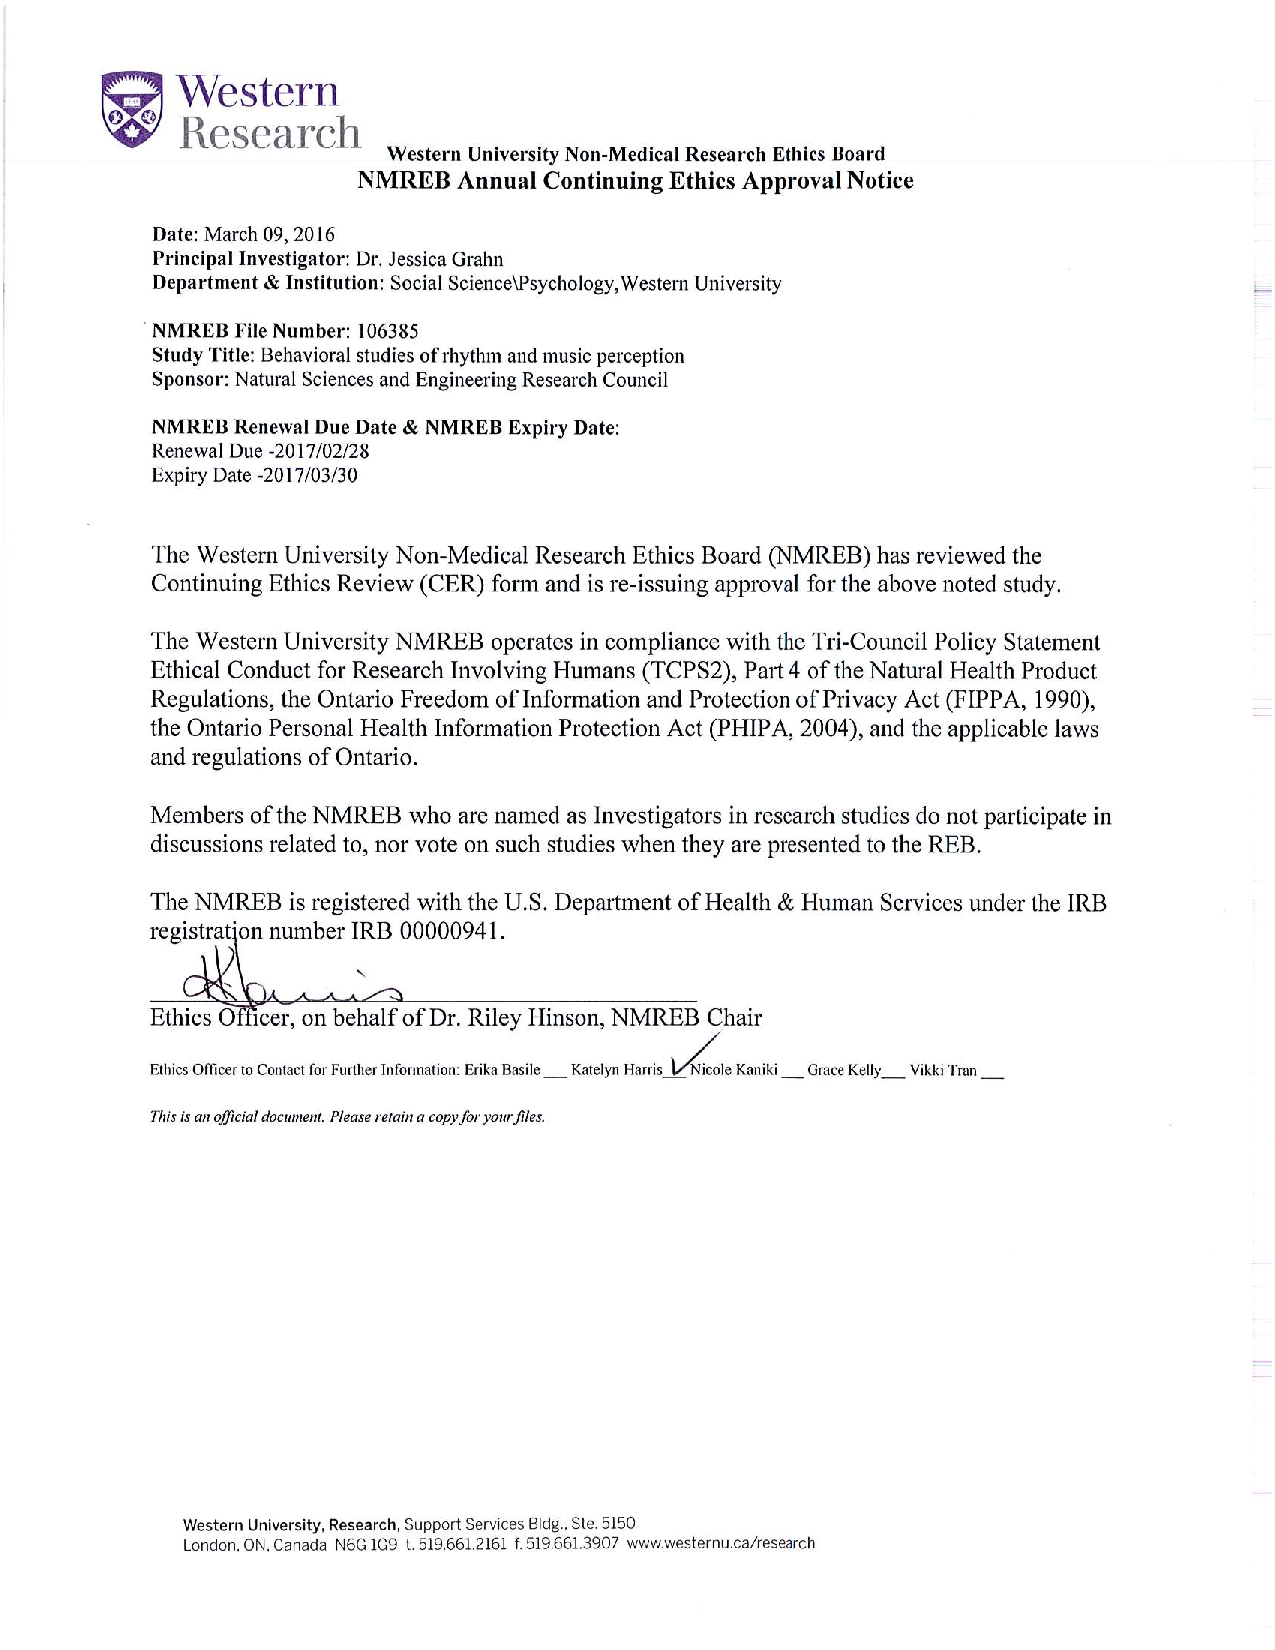
\includepdf{Figures/EthicsApproval.pdf}
\chapter{Questionnaire}\label{appendix:questionnaire}
\myappendices{Appendix \ref{appendix:questionnaire} {Questionnaire}}

The questionnaire used during both the EEG and the behavioural experiment can be found on the following pages.
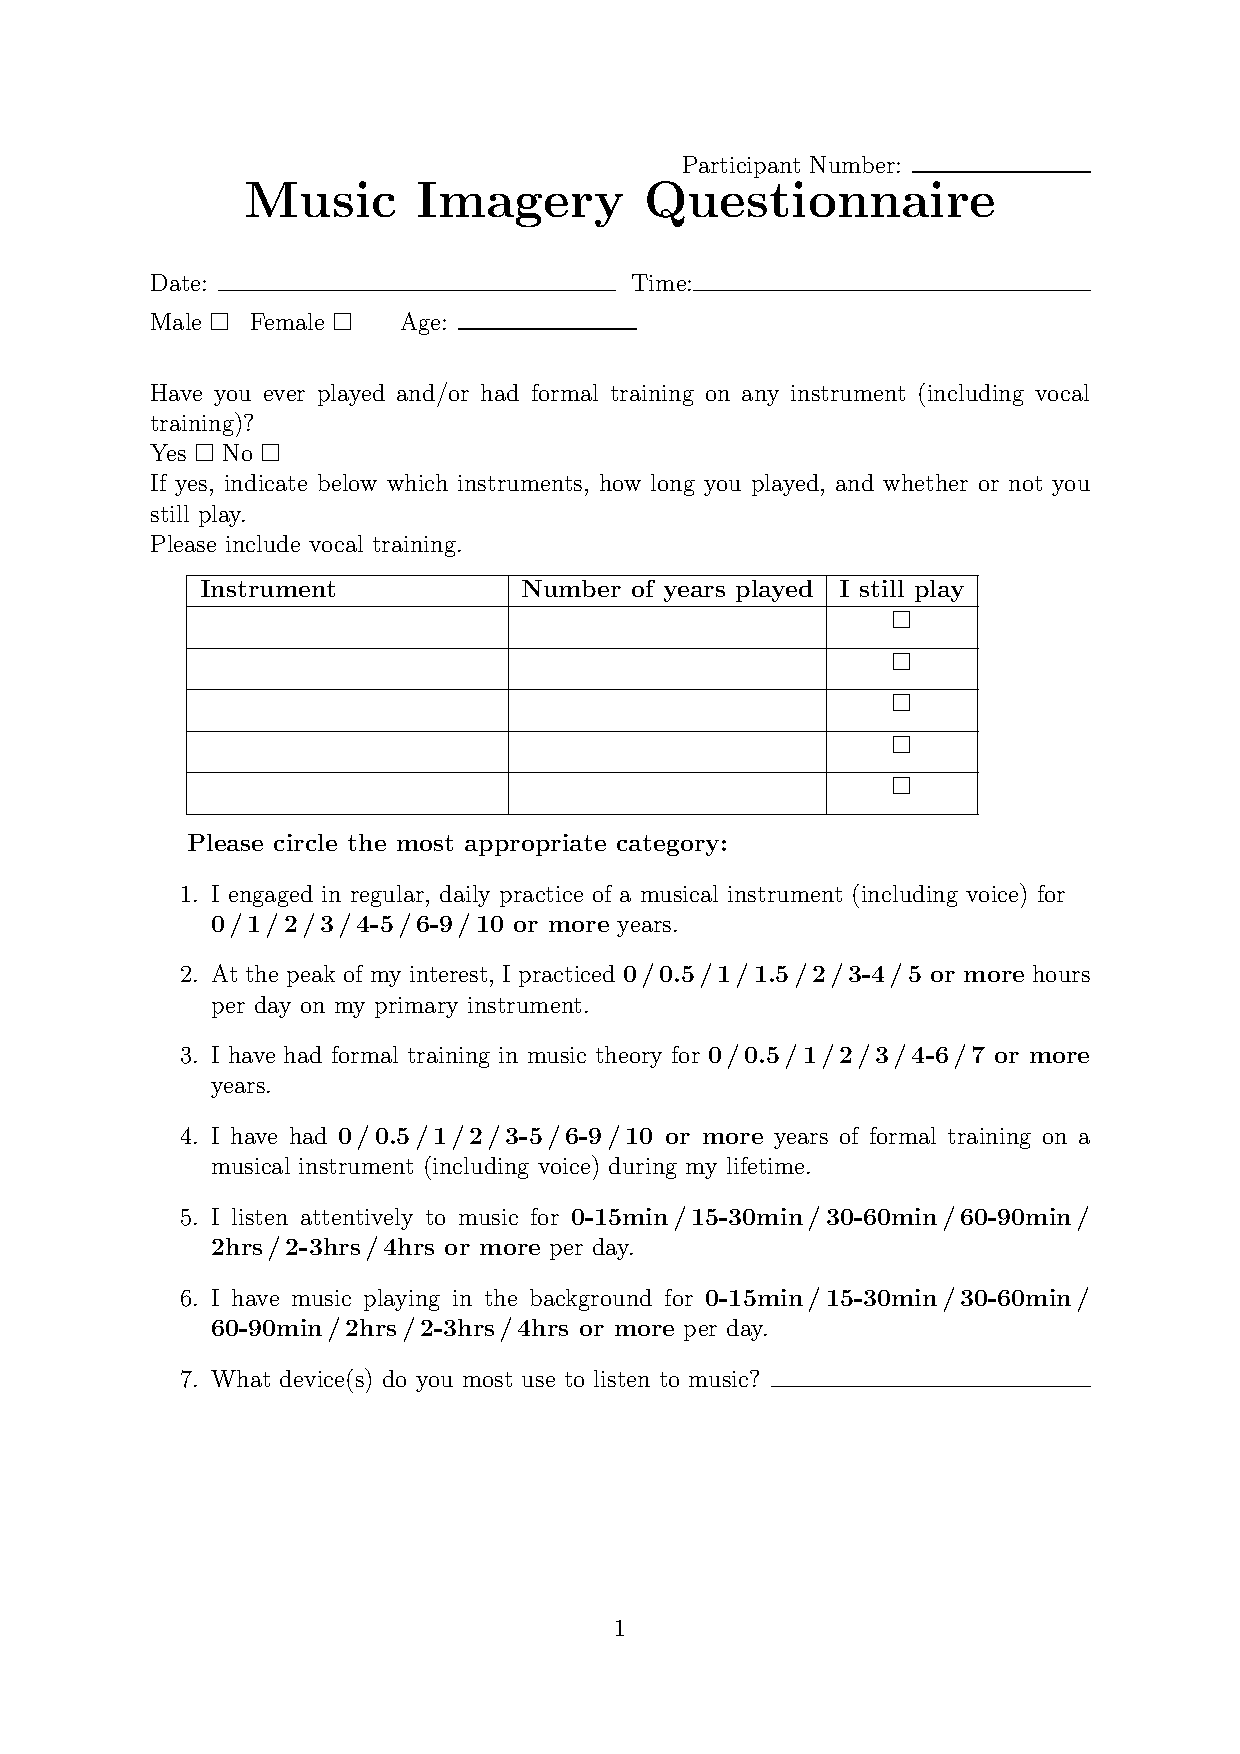
\includepdf[pages={1,2}]{Figures/questionnaire.pdf}

\end{appendices}

%CV only relevant stuff... not full CV.
\addcontentsline{toc}{chapter}{Curriculum Vitae}
\chapter*{Curriculum Vitae}
%\begin{table}[ht]
%\begin{tabular}{ll}
%\textbf{Name:} & \firstname{} \lastname\\\\
%\textbf{Post-Secondary} & La La School\\
%\textbf{Education and}& La La Land\\
%\textbf{Degrees:}& 1996 - 2000 M.A.\\\\
%& University of Western Ontario\\
%& London, ON\\
%& 2008 - 2012 Ph.D.\\\\
%\textbf{Honours and}& NSERC PGS M\\
%\textbf{Awards:}& 2006-2007\\\\
%\textbf{Related Work}& Teaching Assistant\\
%\textbf{Experience:}& The University of Western Ontario\\
%& 2008 - 2012\\
%\end{tabular}
%\end{table}
%\subsubsection*{Publications:}
%La La
\end{document}

